\documentclass[11pt]{article}

\usepackage{color}
\usepackage{amsmath,amsthm,amssymb,multirow,paralist}
\usepackage{graphicx}

% Use 1/2-inch margins.
\usepackage[margin=1in]{geometry}
\usepackage{hyperref}

\begin{document}

\begin{center}
{\Large \textbf{COM S 673: Advanced Topics in Computational Models of Learning\\
Assignment \#1}}\\
\linethickness{1mm}\line(1,0){500}\\
\begin{enumerate}
\item You need to submit a report and your code to
Canvas. Your hard-copy report should include (1) answers to the
non-programming part, and (2) analysis and results of the
programming part. Please put all your code files and report into a compressed file
named ``HW\#\_FirstName\_LastName.zip''
\item Unlimited number of submissions are allowed and the latest one will be timed and graded.
\item Please read and follow submission instructions. No exception will be made to accommodate incorrectly submitted files/reports.
\item All students are required to typeset their reports using latex.
\item Only write your code between the following lines. Do not modify other parts.

\#\#\# YOUR CODE HERE

\#\#\# END YOUR CODE
\end{enumerate}
\end{center}
\linethickness{1mm}\line(1,0){500}

%%%%%%%%%%%%%%%%%%%%%%%%%%%%%%%%%%%%%%%%%%%%%%%%%%%%%%%%%%%%%%%%%%%%%%%%%%%%%%%

%%%%%%%%%%%%%%%%%%%%%%%%%%%%%%%%%%%%%%%%%%%%%%%%%%%%%%%%%%%%%%%%%%%%%%%%%%%%%%%

\textbf{Linear Models for Handwritten Digits Classification}: In this assignment, you will implement the binary logistic regression model and multi-class logistic regression model on a partial dataset from MNIST. In this classification task, the model will take a $16 \times 16$ image of handwritten digits as inputs and classify the image into different classes. For the binary case, the classes are 1 and 2 while for the multi-class case, the classes are 0, 1,  and 2.
The ``data'' fold contains the dataset which has already been split into a training set and a testing set.  All data examples are saved in dictionary-like objects using ``npz'' file.  For each data sample, the dictionary key `x'  indicates its raw features, which are represented by a 256-dimensional vector where the values between $[-1, 1]$ indicate grayscale pixel values for a $16 \times 16$ image. In addition, the key 'y' is the label for a data example, which can be 0, 1, or 2.   The ``code'' fold provides the starting code. You must implement the models using the starting code.

\begin{enumerate}

    \item Data Preprocessing [15 points]: In this problem, you need to finish ``code/DataReader.py''.
    \begin{enumerate}
        \item Explain what the function $train\_valid\_split$ does and why we need this step.

        \item Before testing, is it correct to re-train the model on the whole training set? Explain your answer.

        \item In this assignment, we use two hand-crafted features:

        The first feature is a measure of symmetry. For a $16 \times 16$ image $x$, it is defined as
        $$F_{symmetry} = -\frac{\sum_{pixel}{|x - flip(x)|}}{256},$$
        where $256$ is the number of pixels and $flip(\cdot)$ means left and right flipping.

        The second feature is a measure of intensity. For a $16 \times 16$ image $x$, it is defined as
        $$F_{intensity} = \frac{\sum_{pixel}{x}}{256},$$
        which is simply the average of pixel values.

        Implement them in the function $prepare\_X$.

        \item In the function $prepare\_X$, there is a third feature which is always 1. Explain why we need it.

        \item The function $prepare\_y$ is already finished. Note that the returned indices stores the indices for data from class 1 and 2. Only use these two classes for binary classification and convert the labels to +1 and -1 if necessary.

        \item Test your code in ``code/main.py'' and visualize the training data from class 1 and 2 by implementing the function $visualize\_features$. The visualization should not include the third feature. Therefore it is a 2-D scatter plot. Include the figure in your submission.
    \end{enumerate}


    \item Cross-entropy loss [20 points]: In logistic regression, we use the cross-entropy loss.
    \begin{enumerate}
        \item Write the loss function $E(w)$ for one training data sample $(x, y)$. Note that the binaray labels are $1$ and $-1$.

        \item Compute the gradient $\nabla E(w)$. Please provide the intermediate steps.

        \item Once the optimal $w$ is obtained, it can be used to make predictions as follows:
        \[ \mbox{Predicted class of }x =
        \begin{cases}
        1       & \quad \text{if } \theta(w^Tx)\geq 0.5\\
        -1  & \quad \text{if } \theta(w^Tx)<0.5\\
        \end{cases}
        \]
        where the function $\theta(z)=\frac{1}{1+e^{-z}}$ looks like
        \begin{center}
            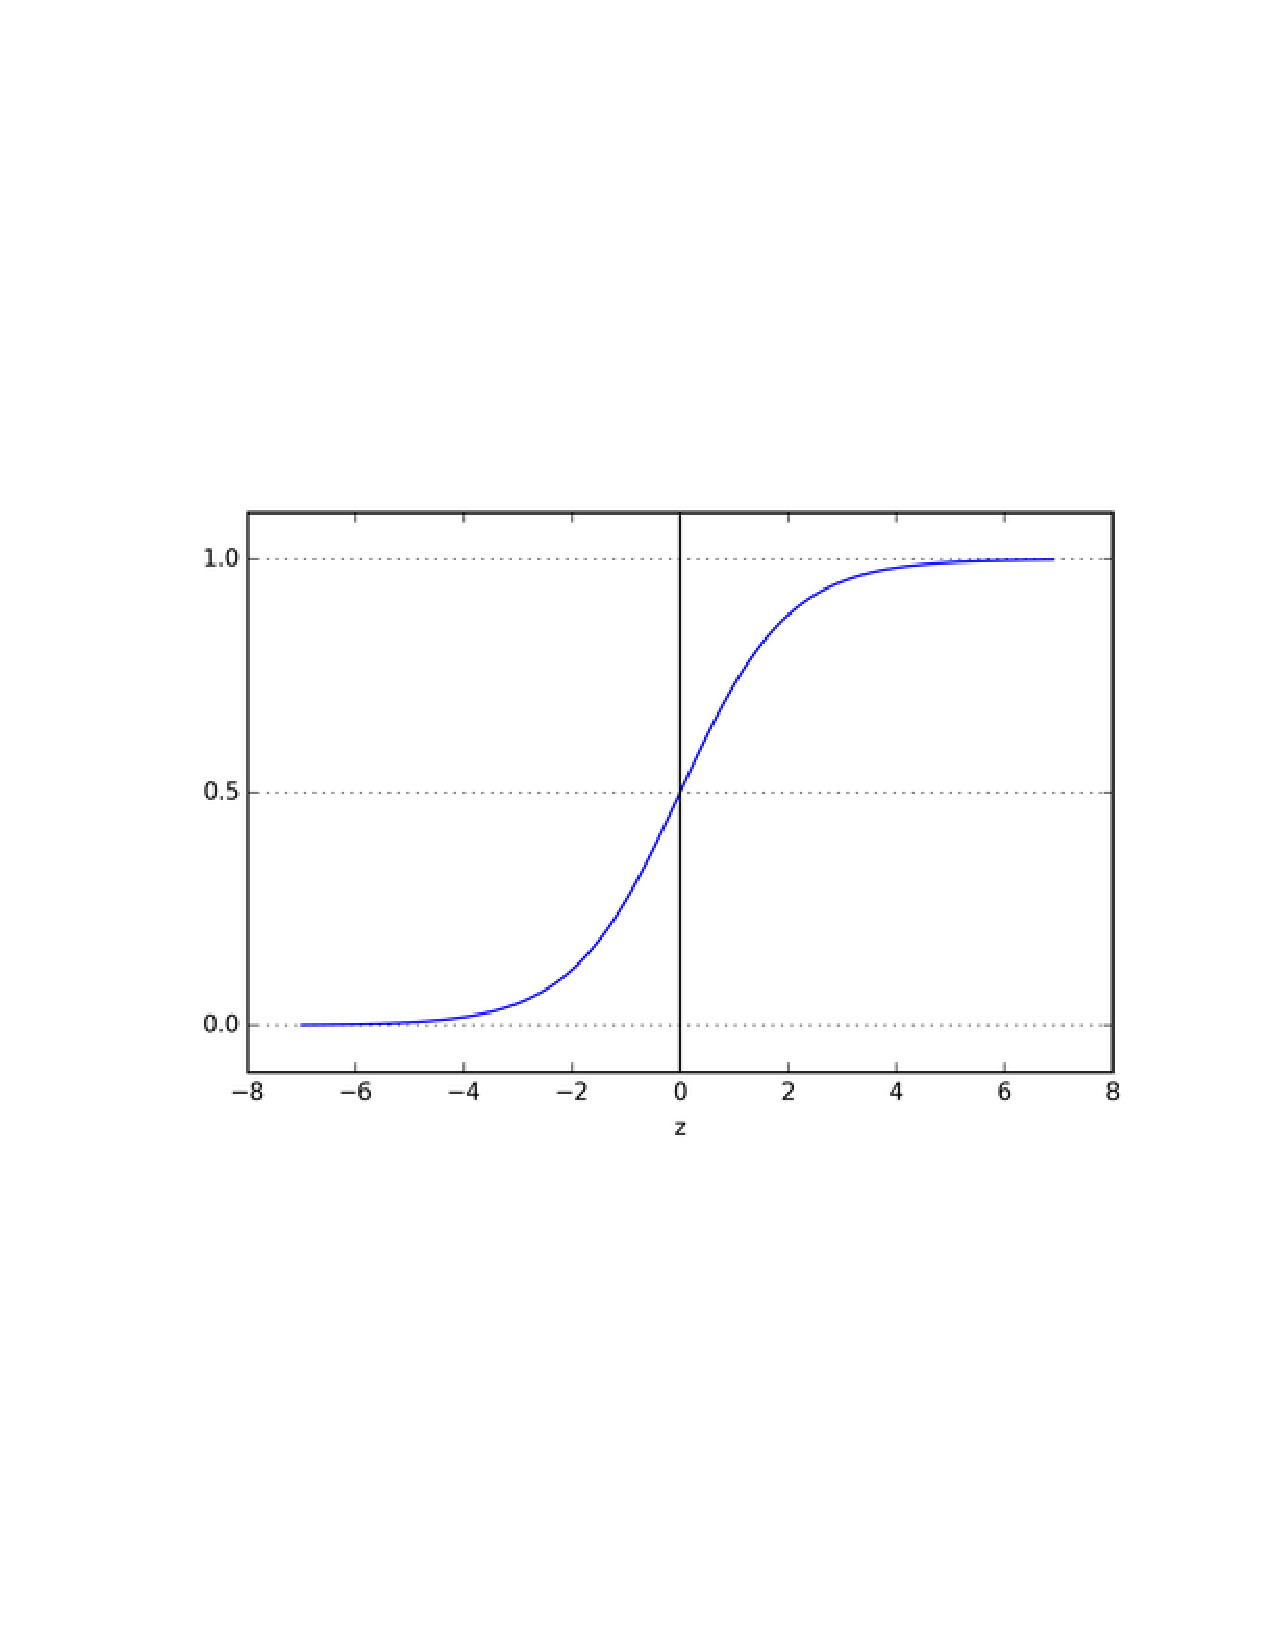
\includegraphics[width=5cm]{sigmoid.pdf}
        \end{center}
        However, this is not the most efficient way since the decision boundary is linear. Why? Expalin it. When will we need to use the sigmoid function in prediction?

        \item Is the decision boundary still linear if the prediction rule
        is changed to the following? Justify briefly.
        \[ \mbox{Predicted label of }x =
        \begin{cases}
        1       & \quad \text{if } \theta(w^Tx)\geq 0.9\\
        -1  & \quad \text{if } \theta(w^Tx)<0.9\\
        \end{cases}
        \]

        \item In light of your answers to the above two questions, what is the essential property of logistic regression that results in the linear decision boundary?
    \end{enumerate}

    \item Sigmoid logistic regression [25 points]: In this problem, you need to finish ``code/LogisticRegression.py''. \textbf{Please follow the instructions in the starting code. Please use data from class 1 and 2 for the binary classification.}
    \begin{enumerate}
        \item Based on (b) in the last problem, implement the function $\_gradient$.

        \item There are different ways to train a logistic regression model. In this assignment, you need to implement gradient descent, stochastic gradient descent and batch gradient descent in the functions $fit\_GD$, $fit\_SGD$ and $fit\_BGD$, respectively. Note that GD and SDG are actually special cases of BGD.

        \item Implement the functions $predict$ and $score$ for prediction and evaluation, respectively. Additionally, please implement the function $predict\_proba$ which outputs the probabilities of both classes.

        \item Test your code in ``code/main.py'' and visualize the results after training by using the function $visualize\_results$. Include the figure in your submission.

        \item Implement the testing process and report the test accuracy of your best logistic regression model.
    \end{enumerate}

    \item Softmax logistic regression [20 points]: In this problem, you need to finish ``code/LRM.py''. \textbf{Please follow the instructions in the starting code. }
\begin{enumerate}
    \item Based on the course notes, implement the function $\_gradient$.

    \item  In this assignment, you only need to implement  batch gradient descent in the function  $fit\_BGD$.

    \item Implement the functions $predict$ and $score$ for prediction and evaluation, respectively.

    \item Test your code in ``code/main.py'' and visualize the results after training by using the function $visualize\_results\_multi$. Include the figure in your submission.

    \item Implement the testing process and report the test accuracy of your best logistic regression model.
\end{enumerate}


    \item Softmax logistic vs Sigmoid logistic [20 points]: In this problem, you need to experimentally compare these two methods.  \textbf{Please follow the instructions in the starting code.} Use data examples from class 1 and 2 for classification.
\begin{enumerate}
    \item Train the softmax logistic classifier and the sigmoid logistic classifier using the same data until convergence. Compare these two classifiers and report your observations and insights.

    \item Explore the training of these two classifiers and monitor the graidents/weights. How can we set the learning rates so that $w_1-w_2= w$ holds for all training steps?

\end{enumerate}

\end{enumerate}



\end{document}
